\documentclass[a4paper, 12pt]{article}

\usepackage{escexam}

%\excludecomment{solution}

%\renewcommand*\ttdefault{cmvtt}

\begin{document}

\vspace*{14ex}

\makeheader{1}                              					% examination number (used to set theorem, lemma numbers)
           {August 29, 2021}      					         		% examination date or deadline
					 {40}											% total marks
					 {Homework Assignment 1}							% Minor Quiz 1, Major Quiz 2, End sem, etc
					
\begin{tabular}{cl}
%%1. & This question paper contains a total of 12 pages (9 sides of paper). Please verify.\\
%1. & Write your name, roll number, department, section on \textbf{every side of every sheet} of this booklet\\
1. & Write the answers \textbf{neatly} in the given boxes.\\
2. & You may  discuss the solutions with the other students, but you have to write them in your own words.
%%4. & Do not give derivations/elaborate steps unless the question specifically asks you to provide these.
\end{tabular}


\begin{problem}{}
(20 points) Problem 7 in the Exercises of Chapter 2 in [LS15]. 

\noindent
[LS15] Edward A. Lee and Sanjit A. Seshia, Introduction to Embedded Systems, A Cyber-Physical Systems Approach, Second Edition, http://LeeSeshia.org, ISBN 978-1-312-42740-2, 2015. \\
\\
\begin{minipage}{1\textwidth}
		\rectangle{\linewidth}{20cm}
		% \ruledrectangle{7}
\end{minipage}
\newpage
\ \\
\begin{minipage}{1\textwidth}
		\rectangle{\linewidth}{24cm}
		% \ruledrectangle{7}
\end{minipage}
\newpage
\ \\
\begin{minipage}{1\textwidth}
		\rectangle{\linewidth}{24cm}
		% \ruledrectangle{7}
\end{minipage}
\newpage
\ \\
\begin{minipage}{1\textwidth}
		\rectangle{\linewidth}{24cm}
		% \ruledrectangle{7}
\end{minipage}
\end{problem}

\newpage

\begin{problem}{}
(10 points) The states of the linearized model of a vehicle steering system represent the lateral deviation of the vehicle from the x-axis and the angle between the vehicle axis and the x-axis. The output of the linearized model is only the first state. Construct a Simulink model for the vehicle steering system with its controller that includes an observer. The dynamics are available in Example 6.4 and Example 7.3 in [AM09]. Apply a sinusoidal signal as the reference trajectory that specifies the desired deviation of the vehicle from the x-axis with time. Plot the output (lateral deviation of the vehicle from the x-axis) with time. 

\noindent
\noindent
[AM09] K. J. Astrom and R. M. Murray. Feedback Systems: An Introduction for Scientists and Engineers. Princeton University Press, 2009. \\
http://www.cds.caltech.edu/$\sim$murray/books/AM05/pdf/am08-complete\_22Feb09.pdf. \\
\\
\begin{minipage}{1\textwidth}
		\rectangle{\linewidth}{20cm}
		% \ruledrectangle{7}
\end{minipage}
\newpage
\ \\
\begin{minipage}{1\textwidth}
		\rectangle{\linewidth}{24cm}
		% \ruledrectangle{7}
\end{minipage}
\newpage
\ \\
\begin{minipage}{1\textwidth}
		\rectangle{\linewidth}{24cm}
		% \ruledrectangle{7}
\end{minipage}
\newpage
\ \\
\begin{minipage}{1\textwidth}
		\rectangle{\linewidth}{24cm}
		% \ruledrectangle{7}
\end{minipage}
\end{problem}

\newpage


\begin{problem}{}
(10 points)
Consider the following model for a thermostat system.

\begin{center}
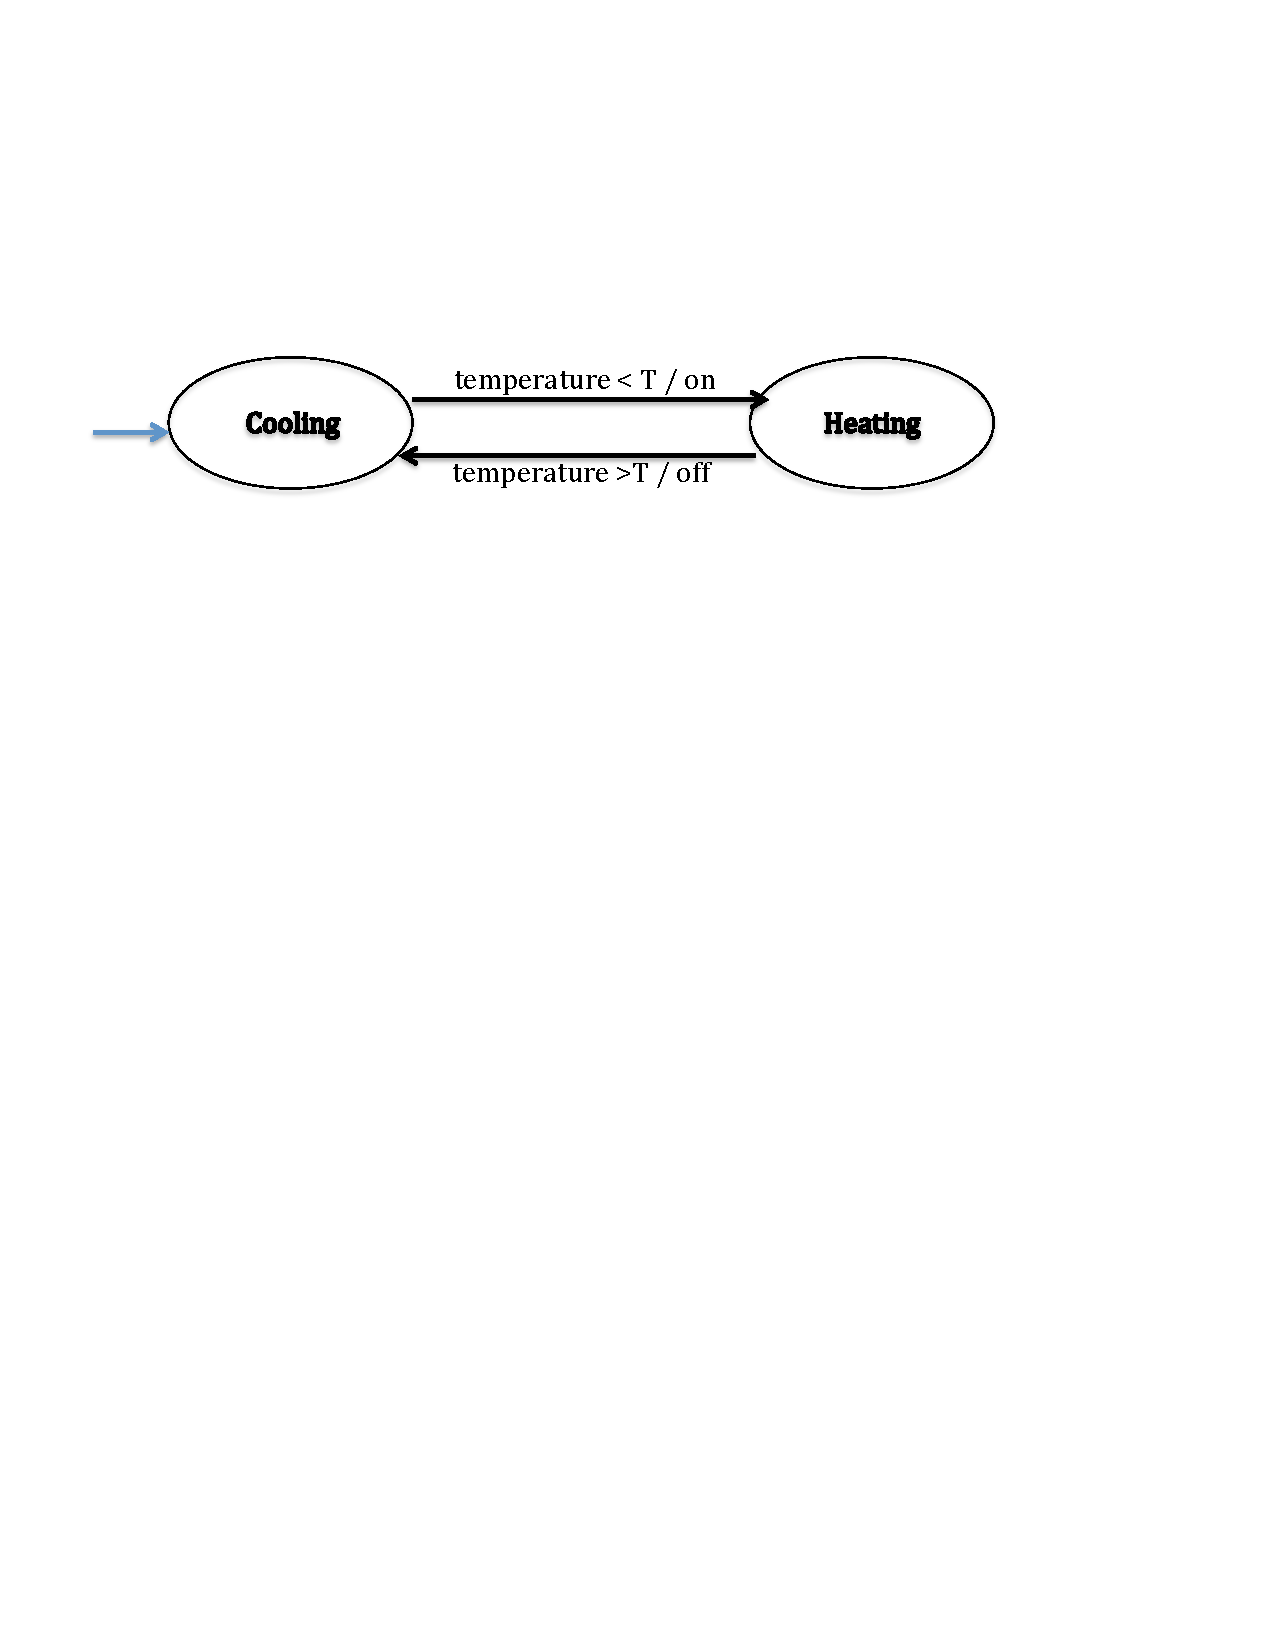
\includegraphics[scale=0.5]{temperature.pdf}
\end{center}

The thermostat has been designed to maintain the temperature of a room at T$^{\circ}$C.
The model has two states: \textit{cooling} and \textit{heating}.
When the system is in the \textit{cooling} state and the temperature of the room goes below T$^{\circ}$C, the system
generates a signal to switch on a heater and moves to the \textit{heating} state. 
When the temperature of the room goes over T$^{\circ}$C, the system generates a signal to switch off the heater and moves to
the \textit{cooling} state.\\
(a) Represent the system as an actor that takes the current temperature as input and produces a signal to control the heater. The actor uses the set point T as a parameter.\\
(b) Identify a design problem in the model.\\
(c) Provide two different remedies to address the problem. \\
(d) Compare your proposed two solutions in terms of ease of implementation and guaranties on the system behavior.  \\\\
\\
\begin{minipage}{1\textwidth}
		\rectangle{\linewidth}{16cm}
		% \ruledrectangle{7}
\end{minipage}
\newpage
\ \\
\begin{minipage}{1\textwidth}
		\rectangle{\linewidth}{24cm}
		% \ruledrectangle{7}
\end{minipage}
\newpage
\ \\
\begin{minipage}{1\textwidth}
		\rectangle{\linewidth}{24cm}
		% \ruledrectangle{7}
\end{minipage}
\newpage
\ \\
\begin{minipage}{1\textwidth}
		\rectangle{\linewidth}{24cm}
		% \ruledrectangle{7}
\end{minipage}
\end{problem}
\newpage


%\toptitlebar
%\begin{center}
%	BLANK SPACE: Any answers written here will be left ungraded.\\ No exceptions.\\ You may use this space for rough work.
%\end{center}
%\begin{figure}[h!]
%\includegraphics[width=\columnwidth]{watermark.png}%
%\end{figure}

\end{document}